\chapter{Basic Conceptual framework}

\section{Content}

Since late 20th Century to Present, China's rapid economic growth 
has been accompanied by significant technological advancements, 
especially in sectors like telecommunications, electronics, 
manufacturing, and space exploration. Furthermore, China has 
emerged as a leader in areas such as 5G technology, e-commerce, 
artificial intelligence, and renewable energy.

\begin{center}
    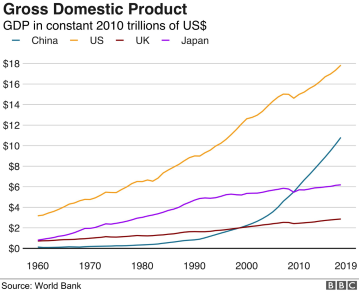
\includegraphics{GrossDomesticProduct.png}
\end{center}

The 1950s had seen one of the biggest human disasters of the 20th 
Century. The Great Leap Forward was Mao Zedong's attempt to rapidly 
industrialize China's peasant economy, but it failed and 10-40 
million people died between 1959-1961 - the most costly famine 
in human history.

This was followed by the economic disruption of the Cultural 
Revolution in the 1960s, a campaign which Mao launched to rid the 
Communist party of his rivals, but which ended up destroying much 
of the country's social fabric.Yet after Mao's death in 1976, 
reforms spearheaded by Deng Xiaoping began to reshape the economy. 
Peasants were granted rights to farm their own plots, improving 
living standards and easing food shortages.

The door was opened to foreign investment as the US and China 
re-established diplomatic ties in 1979. Eager to take advantage of 
cheap labour and low rent costs, money poured in. "From the end of 
the 1970s onwards we've seen what is easily the 
most impressive economic miracle of any economy in history," says 
David Mann, global chief economist at Standard Chartered Bank.

Through the 1990s, China began to clock rapid growth rates and joining 
the World Trade Organization in 2001 gave it another jolt. Trade 
barriers and tariffs with other countries were lowered and soon 
Chinese goods were everywhere.

\section{Basic Conceptual framework}

China's government plays a significant role in shaping the technology 
landscape. It implements policies and initiatives to support research 
and development, innovation, and the growth of technology companies. 
Key elements include the "Made in China 2025" plan and the "Belt and 
Road Initiative.". China has numerous state-owned enterprises in various 
industries, including technology. These SOEs receive substantial 
government support and play a crucial role in China's technological 
development.

China's private sector has become a major driver of innovation, with 
companies like Alibaba, Tencent, and Huawei at the forefront. These 
firms invest heavily in research and development and are expanding 
globally. China has developed technology clusters and innovation 
ecosystems in cities like Beijing, Shanghai, Shenzhen, and Hangzhou. 
These regions have attracted talent, capital, and companies, fostering 
innovation and entrepreneurship. China is increasing its investment in 
research and development, leading to advancements in areas like artificial 
intelligence, biotechnology, and renewable energy. Universities and 
research institutions are also contributing to technological progress.

China is known as the "world's factory" due to its robust manufacturing 
capabilities. The country's supply chain infrastructure supports the 
production of a wide range of technology products. Chinese technology 
companies are expanding globally, exporting their products and services, 
and investing in overseas markets. This globalization has geopolitical 
and economic implications. China has implemented regulations governing 
technology and data privacy, such as the Cybersecurity Law and the 
Personal Information Protection Law, which impact the way technology 
companies operate.